%!TEX root=../ctl-phd-thesis.tex

\section{Abstract}
\par As biologists discover and learn to embrace the complexity of biological systems, computational data analysis and modeling have become critical for furthering our understanding. Exascale computing will enable the development of new predictive multiscale models, transforming how we study the behaviors of organisms and ecosystems, ultimately leading to new innovations and discoveries.

\section{Introduction}
\par Computers have completely revolutionized the way we study and understand the complexity and multiscale nature of biology. From simulating the bond making and breaking of enzyme catalysis to computing protein sequence alignments, nearly every aspect of modern biology has some level of computation involved. There has been a clear trend throughout history of algorithmic and hardware advances creating new opportunities for biologists. In the early days, computers were used to accelerate difficult tasks, such as the determination of structures from X-ray diffraction data, as well as to piece together full gene sequences from sequence fragments. This spurred an era of uncovering the molecular basis of biology. Since then, drastic improvements in computing power and automation have enabled the rapid creation of large structural and sequence datasets such as the Protein Data Bank and the Human Genome Project\cite{Berman2000,InternationalHumanGenomeSequencingConsortium2004}. At the same time, owing to the development of numerical integration techniques and improvements in our understanding of chemical and biological physics, scientists began developing complicated models and simulations of various phenomena. Without the driving force of computation, our understanding of biology simply would not be as advanced as it is today. Even the latest structural biology ``revolution,'' cryoelectron microscopy (CryoEM), is only possible because of the ability to store and process massive imaging datasets using computers\cite{Callaway2015a}. The marriage of computation and biology has completely changed our understanding of life and revolutionized medicine. This trend where innovations in biological research piggyback off advances in computation will continue. Efforts such as the Exascale Computing Project (ECP) spearheaded by the National Strategic Computing Initiative (NSCI) promise to reduce the time to deployment of the next generation of exascale supercomputing facilities, and we predict that this will have a transformative effect on computational biology.

\par The ultimate goal of computational biology is to develop the ability to predict, control, and design the function of organisms and biomes. We seek to understand, through the discovery and characterization of networks of biochemical and chemical linkages/reactions defining metabolism and other relevant chemistries, how perturbations such as the introduction of a drug or changing environmental conditions will affect an organism or population. Despite decades of experimental parameter collection, our ability to model across spatiotemporal scales to predict emergent system behaviors remains unrealized. Existing efforts have been confounded by both the need to account for phenomena that occur over 15 and 10 orders of temporal and spatial magnitude, respectively, as well as the need to accurately account for physiological or genetic variability in the population. Combating these factors, biologists have turned toward increasingly quantitative and data-driven methods to identify anomalies and query behaviors of interest. Through a combination of clever experimental design and technological innovation, experiments such as sequencing, structural imaging, and molecular functional assays are being automated. The trends of the past several years indicate that the output data rates and data sizes of these technologies are growing at an exponential rate. To convert these raw data streams into useful information such as genes and genomes, protein and cellular ultrastructures, and chemical activities, computationally intensive algorithms that require high memory and disk space are employed. To keep up with the flood of data, in the future, biologists will need access to suitable new computing resources such as exascale high-performance computing (HPC). Future research into algorithms that scale into exascale will enable the development of data assimilation workflows, and strategies for interconnecting different simulation modalities to enable predictive multiscale systems biology.

\par Exascale computing refers to the development of computing systems that are 1,000 times faster than existing petaflop machines, capable of the sustained delivery of at least 1 exaflop ($10^{18}$ calculations per second). Note that while FLOPs were historically the biggest cost in HPC, in today's post-Moore's law era, the primary design constraint will be system power usage. In our current technology, the cost of data movement is far greater than compute capability. In essence, exascale HPC will likely provide exponential gains in concurrency and parallelism with only modest gains in memory scaling. Nevertheless, these resources, coupled with other compute modalities, will help computational biologists address several of the fundamental challenges we face on a routine basis:
\begin{itemize}
  \item insufficient model/analysis throughput;
  \item insufficient simulation domain or detail;
  \item incomplete model physics;
  \item lack of uncertainty quantification; and
  \item lack of workflows that are able to reproducibly and robustly integrate simulation, experimental data, and analytics.
\end{itemize}
\par By tackling these roadblocks, exascale computing will create new opportunities to develop more realistic simulations and derive new insights from large datasets. Such advances stand to transform what we understand about the -omics fields (genomics, metagenomics, proteomics, metabolomics, and so on), evolutionary biology, personalized medicine, and drug discovery.


\section{Keeping Pace with Data}

\par Improvements in technology and automation have led to the creation of enormous streams of experimental data. For example, advances such as next-generation sequencing have driven down the costs of sequencing whole genomes to an affordable level. Efforts are already underway to deep sequence millions of human genomes\cite{Kaiser2016}, while others seek to sequence thousands of non-human organisms across all domains of life\cite{Pennisi2017,Normile2017}. What comes out of the sequencer is not an ordered genome sequence but rather the sequences of billions of short fragments (multiple terabytes). Biologists must then use complex genome assembly algorithms, which compare and align these fragments to assemble the complete genome. This is a classical bioinformatics task that can require up to several terabytes of memory\cite{Nystedt2013}. Although the genome assembly problem traditionally necessitates a tightly coupled (HPC) compute infrastructure due to the algorithmic communication load\cite{Spjuth2016}, some have developed MapReduce-based algorithms to run in the cloud\cite{ODriscoll2013}. Additional research in the future will be necessary to determine whether the flexibility of elastic cloud computing at the sacrifice of increased network communication latency will be preferred by the community.
\par Once the genome is assembled, biologists can use computationally driven comparative analysis to correlate mutations with diseases and to track the evolutionary (phylogenetic) history of life. Here the computation typically requires pairwise comparisons between genomes or genes. Therefore, the computational effort scales quadratically with respect to the number of available sequences. As the number of complete genomes grows exponentially, exascale computing and other compute modalities can provide the necessary throughput to support these analyses. A philosophical question arises as to whether to store the data in a single resource or distribute it in the cloud. Benefits of localization include reduced network traffic and potentially superior dataset security and provenance. On the other hand, cloud solutions provide superior flexibility for sporadic compute loads. Biologists must work together to develop best practices to protect private patient data as well as to track the software and hardware versions in data processing steps.
\par Beyond this, other important questions remain. Predicting and annotating the functions of genes in genomic and metagenomic sequences will be an ongoing challenge. With sufficient annotation coverage, the metabolism of new organisms can be automatically modeled to predict its functional behaviors. Given the extreme dimensionality of biochemical networks, throughput from exascale computing will be necessary to perform the parameter estimation and optimization of the generated metabolic model. This could lead to the discovery of significant genes that encode proteins that might be useful in biomanufacturing and other industries. Genomics and metagenomics are just two of the many -omics fields that will benefit from exascale resources. In each field, significant discoveries are likely hidden within the datasets. Exascale computing will be key to accessing these discoveries, potentially creating entirely new fields of study.
\par Another source of biological big data stems from continually improving imaging modalities. This includes both medical image sources such as MRI and CT, as well as those employed in life sciences research efforts. Emerging methods such as serial blockface scanning electron microscopy (EM), where the face of a resin embedded tissue block is sequentially imaged using a scanning electron microscope as thin veneers of tissue are removed from the face using an ultramicrotome, will provide unprecedentedly high-resolution 3D views into the ultrastructure of tissue samples\cite{Denk2004}. With automation, in a single run, serial block EM machines can collect data for days at a time resulting in image datasets that are each petabytes in size. Once these datasets are developed, the myriad tissue components in the images must be ``segmented'' (that is, traced and labeled) for subsequent analysis (see Figures \ref{fig:cruworkflow}(a)–(d)). Owing to the huge number of collected images, human-driven manual segmentation will be impossible for future datasets. Computational biologists will need to develop methods, likely similar to deep-learning-based computer vision algorithms, to automatically segment tissue features. Furthermore, as the throughput and resolution of imaging increases, our ability to move and interact with the image data will be reduced. To minimize movement of data, imaging instrumentation can be directly connected to upcoming HPC resources for both processing and visualization. Exascale computers will allow biologists to use large and complex neural network architectures, which require high memory to process the data with minimal down sampling.
\par In addition to the benefits of increased computational throughput and parallelism, biological big data will also benefit from the many other architectural improvements necessary to support exascale. Improvements to memory architectures and interconnects might lead to faster data accessibility. When coupled with the increased throughput, exascale technology will support new advanced interactive analysis for large data sets (for example, in the image data segmentation and refinement example given above). Additionally, new workflows and strategies for data handling and provenance tracking will help address the data storage crisis many labs are facing today. As datasets grow in size, biologists might turn to on-the-fly processing, similar to what is done in the high-energy physics community, to extract parameters of interest during runtime, discarding raw data instead of saving it for postprocessing.

\begin{figure}
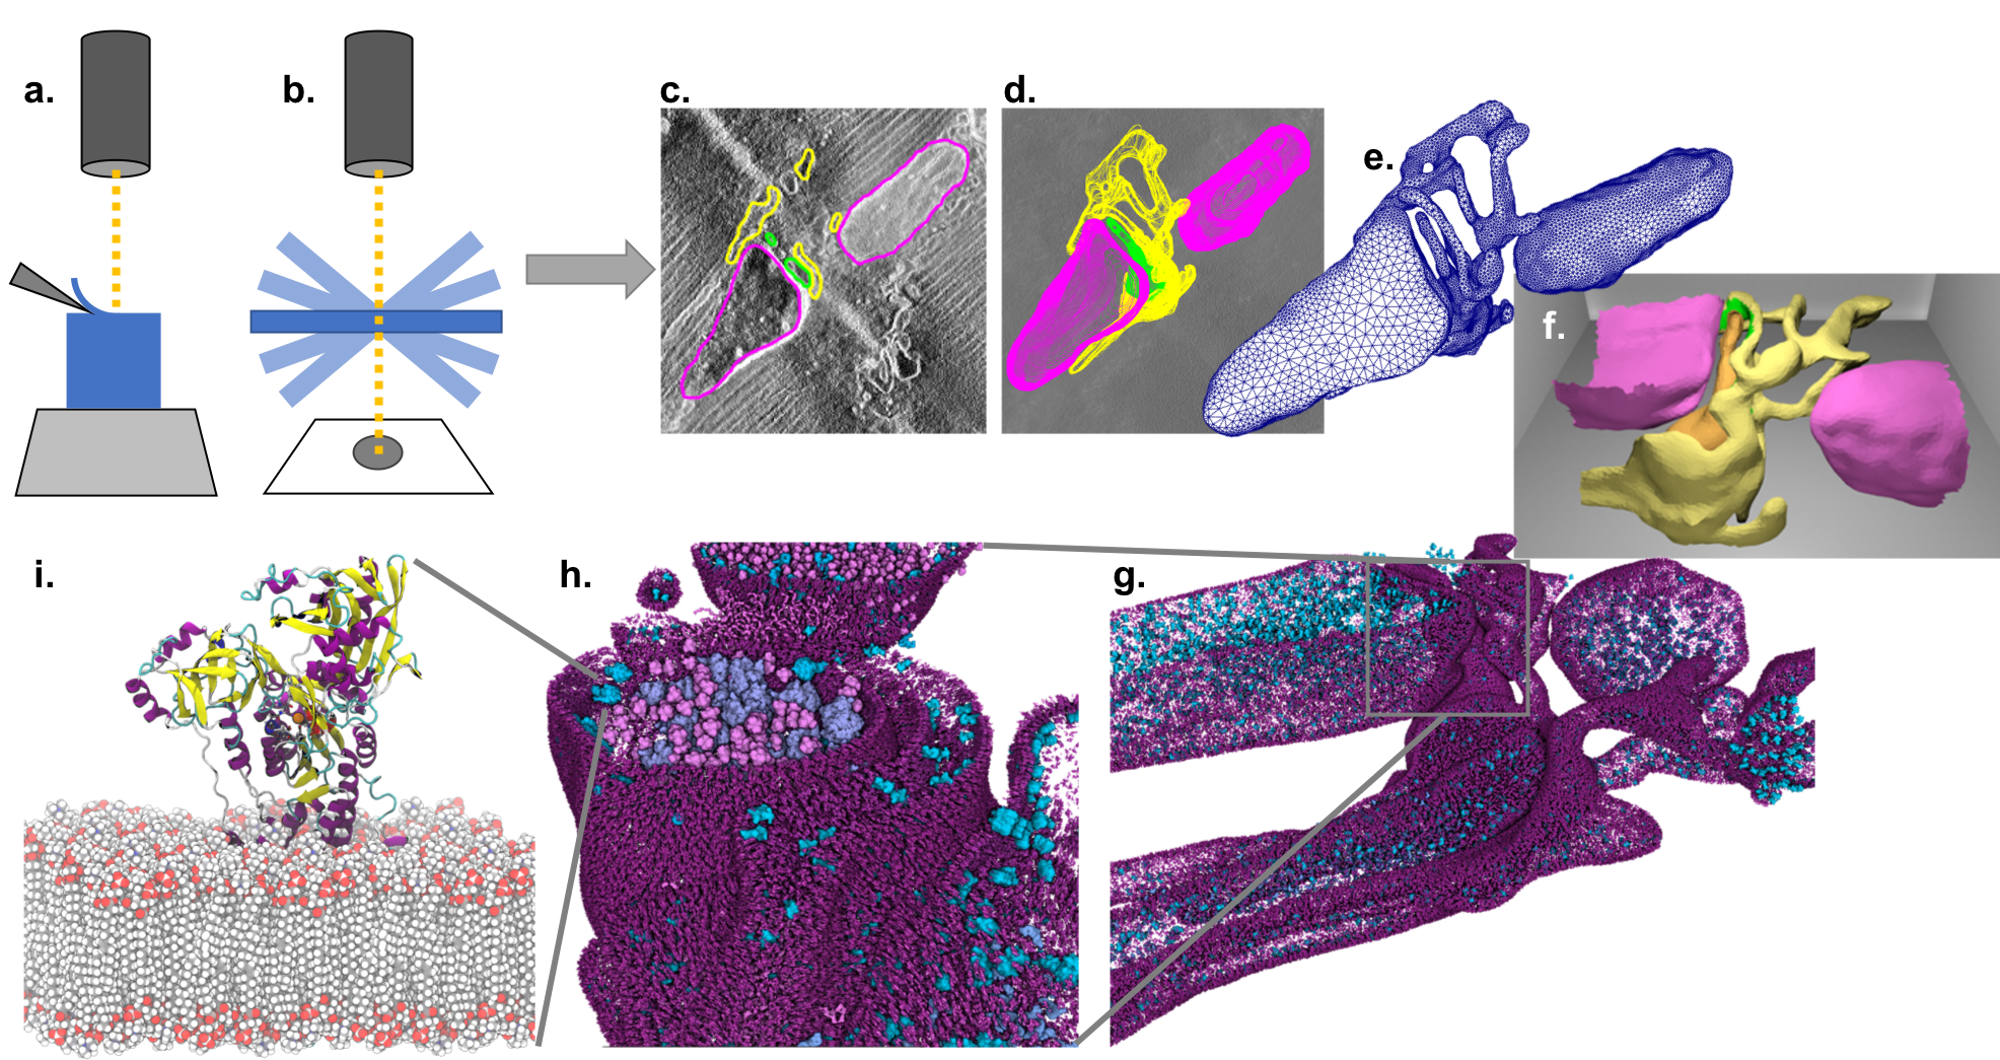
\includegraphics{./Figures/CRU_Workflow.png}
\caption{Exascale computing will aid the process of bringing to life the multiscale modeling of complex molecular scenes. Starting from volume microscopy modalities such as (a) serial block-face scanning electron microscopy and (b) electron tomography, biologists can gain unparalleled views into the cellular ultrastructure. (c) Biological features in the collected images are segmented and visualized as (d) stacks of contours. (e) Using mesh generation algorithms, computable representations of the geometries can be generated. (f) Boundaries of a scene are marked to represent specific boundary conditions. (g) Using cellPACK, the mesh geometry can be filled with molecular-level details. (h) Zooming in, many different diverse membrane and cytosolic proteins interact within this subcellular space. (i) Individual membrane and cytosolic proteins can be modeled using atomistic techniques such as molecular dynamics and Brownian dynamics to derive relevant model parameters. The computed parameters from these isolated models can be integrated up into models of the cellular scene.}
\label{fig:cruworkflow}
\end{figure}

\section{Supercharging Biomolecular Simulations}
\par As we uncover new protein sequences, there will be a growing need to determine their structures. Protein structures are helpful to biologists for inferring protein function as well as for predicting protein-protein interactions that are critical for system feedback and regulation. Moreover, structures are integral for modern structure-based drug discovery efforts. Due to the extreme cost and difficulty of experimental structural genomics pipelines, computational methods for predicting protein folds can be used as a supplement. Protein structure prediction methods such as Rosetta use a Monte Carlo algorithm to generate folding configurations that are then evaluated for energetic stability\cite{Huang2016}. Because proteins are long polymers of amino acids, each with several degrees of freedom, the fold space of proteins is astronomical. Many computations are necessary to enumerate enough folding configurations to generate reliable structure predictions. Large-scale efforts for automated structure prediction, such as the Human Proteome Project and Microbiome Immunity Project driven by IBM's World Community Grid ($\sim$1 PFLOPS), are already ongoing. Protein structure prediction methods tend to be CPU intense with limited storage and I/O requirements. Exascale computers, along with other compute modalities, can provide the throughput necessary to keep pace with the incoming surge of new sequences to fold.
\par With the maturation of protein structure prediction methods, the engineering and design of completely new (de novo) functional proteins should be possible. Since proteins are naturally ``designed'' through evolution, and evolution proceeds by incremental mutation and selection, naturally occurring proteins do not span sequence space. By inferring the timeline of mutation acquisition, scientists can actually trace back the evolution of protein families. There remains a huge set of protein sequences that are not represented by these families\cite{Huang2016}. Using computational protein structure prediction methods, scientists can sample this unknown space of protein sequences and structures, which might hold solutions to challenges in modern biology, medicine, and nanotechnology. Again, the concurrency afforded by exascale resources in tandem with other compute modalities will allow biologists to enumerate new protein sequences, increasing innovation in de novo protein design and decrease time to market for discoveries.
\par Exascale will also benefit other modeling efforts across all scales in computational biology and chemistry. One method, virtual screening, predicts the binding strengths and orientations of libraries of candidate drug molecules to targets of interest. With increased parallelism, researchers will be able to dock increasingly large and diverse sets of compounds, accelerating drug discovery. For applications such as biomolecular simulations, which typically integrate sets of differential equations to generate trajectories of how systems move in time, exascale computing enables the generation of longer simulations and more replicates, improving statistics. One popular method, molecular dynamics (MD), is used to classically simulate atomistic models of macromolecules. MD is often used to identify biological mechanisms of enzyme function, reveal druggable cryptic pockets, or provide computational assays to predict biophysical properties such as drug binding\cite{Liu2018,Durrant2011a,DeVivo2016}. To obtain sufficient MD statistics, scientists model extremely idealized versions of biological systems. By introducing additional model complexity, the amount of sampling must also increase. In most cases, conventional Boltzmann sampling will be too inefficient. Instead, biologists will turn to interconnected ensemble-based methods to increase the simulation's coverage. Concurrency provided by exascale computing will allow for the development of superior ensemble methods, enabling biologists to sample additional complexity.
\par Using these methods, scientists will be able to increase the model detail to study the ramifications of glycosylations and other post-translational modifications as well as the impact of physiologically relevant bilayer compositions or polarizable water molecules on drug binding, for example. Moreover, with exascale computing, biologists will be able to move from simulating the dynamics of individual proteins toward the modeling of many proteins or macromolecular complexes as they exist in vivo. Owing to the weak scaling properties of MD, with the appropriate exascale machines and improvements in algorithms, simulations of up to billions of atoms will become tractable. Such efforts are aided by new data integration frameworks such as cellPACK\cite{Johnson2015} that are able to build molecular scale models of complex biological scenes. Exascale computing architectures will play an indispensable role in our ability to ``bring these scenes to life'' with physics-based simulation (see Figures \ref{fig:cruworkflow}(e)–(i)).

\section{Big Data, Multiscale Modeling, and Systems Biology}

\par The ultimate challenge of computational biology is the ability to predict how an organism will behave in response to some stimulus. With sufficiently accurate gene annotations, it will be possible to reconstruct and simulate a whole microorganism's metabolic network. With such a model, scientists will be able to predict the conditions at which an organism can proliferate. This will require repeated simulation of the model while scanning various environmental parameters for both benchmarking and subsequent prediction following a new perturbation. Owing to the large number of metabolic processes in a single organism (including, for example, influences of microorganisms that might reside within a larger organism, similar to the gut microbiome within humans) this task will clearly necessitate the use of exascale (and beyond) resources. Through these metabolic modeling efforts, we might discover how to harness organisms to perform difficult jobs such as detoxifying hazardous environmental waste.
\par Other biological predictions will require more complicated modeling approaches. For example, consider the drug design challenge in which computational biologists seek to maximize a compound's therapeutic effect while minimizing side effects\cite{Amaro2018}. At the smallest scales, quantum mechanical (QM), electronic structure methods can predict the electronic state of electrons and nuclei in molecules. This, at least in theory, provides a strategy for computing all molecular properties with high accuracy, allowing researchers to investigate chemical reactivity. However, due to the limits of computational tractability and the enormous spatiotemporal span of biological problems, no single method is suitable for describing all phenomena. QM calculations are tractable for only tens to thousands of atoms depending upon the level of theory modeled. When faced with the challenge of optimizing the reactivity and specificity of covalent enzyme inhibitors or predicting the rate of enzymatic drug degradation, the drug-enzyme system alone might be hundreds of thousands of atoms in size, far beyond the practical size limitations of QM. To achieve sufficient system sampling, researchers must use other methods, such as the aforementioned MD. Notably, MD employs semi-empirical molecular mechanics (MM) force fields that classically represent molecules, neglecting the electronic structure, and cannot probe chemical reactivity. To resolve this, researchers have developed multiscale hybrid QM/MM approaches in which small regions of high importance (for example, catalytic regions) are modeled using QM while the remainder is represented using MM\cite{VanderKamp2013a}. This kind of approach can bring, for example, a representation of chemical reactivity to MD models of complex subcellular scenes. Concurrency at the exascale will be necessary to efficiently couple the different simulation modalities into one integrated simulation.
\par Multiscale methods, which couple different levels of theory, provide adaptive simulation resolution while balancing practicality. To successfully model biological processes spanning from the atomic to cellular, organ, and, ultimately, organism scales many multiscale coupling schemes must be developed. Returning to our drug discovery example, it is often important to model the binding rates of drugs to proteins. This can be computed using a hybrid MD and Brownian dynamics approach\cite{Votapka2015,Votapka2017c}. Similarly the systemic distribution of drug in the bloodstream can be modeled using computational fluid dynamics (CFD). The rates of increase and decrease in circulating drug concentration due to gastric and cellular absorption respectively can be computed using detailed MD simulations to describe the permeation of drugs across bilayers. MD derived rates can then be propagated into systemic CFD models improving the realism of our model. Again, it is evident that, due to the large number of model subsystems that require tight integration along with the need to execute parameter scans for optimizing unknowns, the concurrency provided by exascale will be required to efficiently couple future multiscale simulations.
\par Exascale computing will also pave the way toward personalized medicine. As medical imaging modalities improve, there are other opportunities, such as in cardiac\cite{Kayvanpour2015,Winslow2012} or cancer\cite{Deisboeck2011} modeling, where realistic patient geometries can be coupled with emerging multiscale systems models, described previously, to predict personalized results\cite{Winslow2012}. Let us consider the case of predicting potential cardiac drug interactions: first, from a patient's genetic sequence we can uncover the mutations to key ion channels responsible for maintaining normal cardiac rhythm. Using molecular modeling, we can study the effect of an introduced drug on the behavior of each channel. The drug-induced perturbations of channel behavior can then be coupled to a cellular action potential model. From an MRI image, we can obtain a 3D picture of the patient's heart geometry. Using algorithms from computer vision and machine learning, we can segment the image and create a computer model of the patient's heart. Propagating results from the cellular action potential model to a tissue model applied on the patient's heart geometry, personalized predictions of drug-cardiac interactions can be realized. Critically, the computational throughput of exascale computing will be necessary to produce predictions such as this in a diagnostically relevant timeframe. By combining structural datasets and experimental measurements with various modeling regimes, scientists can construct new models to predict system-level changes to small perturbations for all manner of problems.

\section{Conclusion}

\par In the coming years, discoveries in biology will be driven by the convergence of improved and increasing experimental data, algorithmic advances, and computational power. Exascale computing will be a necessary development to support the ongoing research efforts of computational biologists. From keeping pace with the rate of experimental data generation to enabling new multiscale multiphysics models of complex biological processes, computational science will continue to evolve and, ultimately, transform biology from an observational to a quantitative science. Continued investments in computing infrastructure will speed up the rate of discovery for life science researchers, thus accelerating discoveries with huge potential impacts in diverse markets and creating new opportunities for improved human health and well-being.

\section{Acknowledgements}
\par \Red{TODO}

\par The authors would like to thank Bryn C. Taylor for critical comments, and Sophia P. Hirakis for assistance in figure preparation. Funding and support was provided by the National Science Foundation through XSEDE supercomputer resources provided via TG-CHE060073N to REA. Funding and support from the National Biomedical Computation Resource was provided through NIH P41 GM103426. CTL was supported in part by a NIH Molecular Biophysics Training Grant T32 GM008326.